\documentclass[sigconf,review,anonymous,nonacm]{acmart}

\usepackage{booktabs}
\usepackage{microtype}
\usepackage{graphicx}
\usepackage{amsmath}
\usepackage{array}

\citestyle{acmnumeric}

\AtBeginDocument{%
  \providecommand\BibTeX{{%
    \normalfont B\kern-0.5em{\scshape i\kern-0.25em b}\kern-0.8em\TeX}}}

\acmConference[ISEC 2027]{Innovations in Software Engineering Conference}{February 2027}{Mumbai, India}
\settopmatter{printacmref=false}
\setcopyright{none}
\acmISBN{}
\acmDOI{}

\graphicspath{{../figures/}}

\newcommand{\proj}[1]{\path{#1}}
\newcommand{\col}[1]{\texttt{#1}}
\newcommand{\mns}{\text{-}}

\begin{document}

\title[How Predictable Are CI Build Failures?]{How Predictable Are CI Build Failures? A Leakage Explicit, Baseline Calibrated Replication on TravisTorrent}

\begin{abstract}
Build outcome prediction has reported strong results on TravisTorrent, but those results depend on what information is available at prediction time and how evaluation preserves time order. We assess prediction at enqueue time on fourteen Java and Ruby projects (43{,}230 builds), using six rolling-origin windows per project and features lagged by build completion. Three autoregressive baselines (previous outcome, last-five failure rate, and logistic regression on history) are compared with five learned detectors using 44 pre-execution features. The baselines reach mean AUROC 0.62--0.63 and mean AUPRC lift 1.41--1.48 over ten primary projects; random forest reaches 0.598, while unsupervised detectors range from 0.517 to 0.548. Paired fold-stratified moving-block bootstrap tests with Holm correction find no learned-detector wins over the last-five rule on AUROC; random forest wins on AUPRC in one project and loses in another. Ablations show that outcome history carries most ranking signal, while telemetry, change, and repository groups add little; repository attributes can reduce supervised performance under temporal drift. At a matched 10\% alert budget, the rules achieve 0.49--0.51 precision against mean prevalence 0.35. A cost sensitivity analysis shows that withholding predicted failures is project-dependent; build skipping trades compute savings against failures detected late. These results support testing simple history baselines before adopting learned CI failure predictors.
\end{abstract}

\begin{CCSXML}
<ccs2012>
<concept>
<concept_id>10011007.10011074.10011099</concept_id>
<concept_desc>Software and its engineering~Software verification and validation</concept_desc>
<concept_significance>500</concept_significance>
</concept>
<concept>
<concept_id>10011007.10011074.10011111.10011113</concept_id>
<concept_desc>Software and its engineering~Software evolution</concept_desc>
<concept_significance>300</concept_significance>
</concept>
<concept>
<concept_id>10010147.10010257</concept_id>
<concept_desc>Computing methodologies~Machine learning</concept_desc>
<concept_significance>300</concept_significance>
</concept>
</ccs2012>
\end{CCSXML}

\ccsdesc[500]{Software and its engineering~Software verification and validation}
\ccsdesc[300]{Software and its engineering~Software evolution}
\ccsdesc[300]{Computing methodologies~Machine learning}

\keywords{continuous integration, build outcome prediction, data leakage, temporal evaluation, concept drift, replication, TravisTorrent, cost model}

\maketitle

\section{Introduction}
\label{sec:intro}

Continuous integration (CI) services run a build for every pushed commit or pull request, and the outcome of that build is the most visible quality signal a team receives during the working day. Because a red build interrupts everyone waiting behind it, a long line of work has asked whether the outcome can be predicted before the build runs, so that doomed builds can be deprioritised, safe builds skipped, or authors warned early~\cite{hassan2006, hassanwang2017, nili2017, xiali2017, chen2020buildfast, jin2020, abdalkareem2021skip, saidani2020, saidani2022, sun2024ravenbuild}. Reported results are often strong. Random forests and boosted trees on change and history features reach accuracies above 90 percent and F1 above 0.8 on TravisTorrent projects in several of these studies.

Three properties complicate build-prediction evaluation. TravisTorrent places pre-execution attributes beside measurements produced during execution~\cite{beller2017travistorrent}; random splits can expose models to nearby builds from the same temporal sequence; and project failure prevalence varies widely, making precision and AUPRC hard to interpret without a baseline. We therefore define an enqueue-time feature boundary, lag history by completion time, evaluate over rolling temporal windows, and compare learned detectors with autoregressive rules.

Our study asks how predictable the next build outcome is under leakage-controlled, forward-in-time evaluation, how much predictive value is already available from completed-build outcomes, and what remaining signal may support operational decisions.

\paragraph{Research questions.}
\begin{description}
  \item[RQ1 (Predictability)] How well do leakage free, pre execution features rank the next build by failure risk, and how much of that ranking quality is already achieved by autoregressive rules that read only the outcomes of finished builds?
  \item[RQ2 (Learned detectors against the rules)] Under rolling origin evaluation with dependence aware inference, does any learned detector, unsupervised or supervised, rank builds significantly better than the autoregressive rules, and on how many projects?
  \item[RQ3 (Feature groups and drift)] Which of four feature groups, outcome history, queue and duration telemetry, change churn, and static repository attributes, carries the signal, and how do drifting repository attributes and prevalence shift affect the learned detectors?
  \item[RQ4 (Operational value)] At a matched alert budget, and under a cost model that prices false alarms, missed failures and the diagnostic value of a failing run, which intervention, if any, does the observed ranking quality support?
\end{description}

\paragraph{Contributions.}
\begin{enumerate}
  \item An explicit, testable instantiation of the standard leakage controlled protocol for the 2016 TravisTorrent schema. It differs from earlier instantiations in three documented ways: history features are lagged by completion time rather than by start order; three retrospective discussion counts are added to the exclusion set; and the observation time of every retained column is stated.
  \item A baseline calibrated replication of build outcome prediction on fourteen projects and 43{,}230 builds, evaluated over six rolling origin windows per project, in which three autoregressive rules are compared with three unsupervised and two supervised detectors under a paired, fold stratified, moving block bootstrap with Holm correction.
  \item A diagnosis of two mechanisms that make learned detectors underperform a one line rule on this data: static repository attributes whose training and test ranges are disjoint act as time proxies under a chronological split, and a variance floor in the reconstruction score turned the autoencoder into a single column novelty flag. Both are measured, and the second is repaired.
  \item A matched operating point comparison and a cost model that separates compute from developer time, prices false alarms from two minutes to one full build, prices the information lost when a failing run is withheld, and evaluates a second scenario, build skipping, in which the cost falls on missed failures. The results are placed on a decision table that maps interventions to the ranking quality they require.
  \item A complete replication package in which every table and figure is regenerated by two scripts from stored results.
\end{enumerate}

The paper is organised as follows. Section~\ref{sec:related} positions the work in the build prediction, CI noise, temporal evaluation and AIOps literatures. Section~\ref{sec:design} describes the data, the leakage boundary, the feature groups, the rolling origin protocol, the scorers, the operating points, the cost models and the inference. Section~\ref{sec:results} answers the four research questions. Section~\ref{sec:discussion} interprets the results and states practical implications. Section~\ref{sec:threats} lists the threats to validity, Section~\ref{sec:repro} the replication package, and Section~\ref{sec:conclusion} concludes.

\section{Background and Related Work}
\label{sec:related}

\subsection{Build outcome prediction}
\label{sec:related-prediction}

Predicting whether a build will pass has been studied since Hassan and Zhang used decision trees on the certification history of a large industrial system~\cite{hassan2006}. The public availability of TravisTorrent~\cite{beller2017travistorrent}, which joins Travis CI build logs with GitHub metadata for over a thousand Java and Ruby projects, produced a cluster of studies around the MSR 2017 mining challenge. Ni and Li cascaded classifiers over TravisTorrent features and reported that the result of the previous build was the most influential feature~\cite{nili2017}. Xia and Li compared nine classifiers on the same data~\cite{xiali2017}. Hassan and Wang built change aware models to let developers avoid stalling on builds that were about to fail~\cite{hassanwang2017}. Saidani and colleagues used evolutionary search~\cite{saidani2020} and, later, sequence models over the time ordered build history~\cite{saidani2022}. Chen and colleagues introduced BuildFast, which adds history aware and failure specific features and, importantly for this paper, argued that earlier studies had evaluated on random splits and reported that in time evaluation lowers the numbers substantially~\cite{chen2020buildfast}. Most recently, Sun, Habchi and McIntosh reported large gains from context, relevance and dependency aware features on an industrial code base~\cite{sun2024ravenbuild}, and Hong and colleagues described how practitioners at Atlassian perceive build failure predictions, emphasising trust, precision at the operating point and the cost of false alarms~\cite{hong2024atlassian}. A systematic review by A\"{i}dasso, Sayagh and Bordeleau covers 97 build optimisation studies and lists outcome prediction and selective execution as the dominant responses to long builds and build failures~\cite{aidasso2025slr}.

Two aspects of this literature motivate the present study. First, several of the strong TravisTorrent results were obtained under protocols that the later work has shown to be optimistic: random or shuffled splits~\cite{nili2017, xiali2017}, and feature sets assembled from every numeric column, which in the 2016 schema includes test counts and durations that are measured after the build has run. Second, the strongest single predictor in nearly every study is the outcome of recent builds. Jin and Servant's build selection work rests on the observation that failures cluster in time: once a build fails, the next builds are much more likely to fail, and once a build passes, the next are likely to pass~\cite{jin2020, jin2022}. A study that omits a rule built on that observation cannot say how much its models add.

\subsection{Build selection and the cost of a wrong prediction}
\label{sec:related-cost}

The operational use of a build outcome predictor is not to abort a build that will fail. A failing build is the diagnostic that tells the developer what broke; withholding it destroys that information and the build must eventually run anyway. The interventions actually studied are build and commit skipping~\cite{abdalkareem2021skip, abdalkareem2021ml, jin2020, jin2022}, where predicted passing builds are not run and the cost falls on failures that are observed late; build prioritisation and early feedback~\cite{hassanwang2017}; and, at a finer granularity, test selection and prioritisation in CI~\cite{elbaum2014}. Jin and Servant frame the trade off as builds saved against failures missed and show that the ceiling of any selection method is set by how many failures it is willing to observe late~\cite{jin2022}. Hilton and colleagues quantified the compute and time cost of CI in open source projects~\cite{hilton2016}, and Hong and colleagues report that at Atlassian the acceptability of a predictor was determined by its false alarm rate rather than by its accuracy~\cite{hong2024atlassian}. The cost model in this paper follows this literature: it prices false alarms, missed failures and lost diagnostics separately, sweeps the false alarm cost over a realistic range, and evaluates the skip scenario as well as the withhold scenario.

\subsection{Noise in build outcome labels}
\label{sec:related-noise}

The label available in TravisTorrent is the Travis status of a build. Gallaba and colleagues showed that a substantial share of Travis breakages are caused by jobs that the project has marked as allowed to fail, by environmental problems and by inconsistent statuses across jobs of the same build~\cite{gallaba2018}. Ghaleb and colleagues classified over half of the breakages in a 350{,}000 build sample as noisy, environmental, cascading or allowed, and showed that conclusions drawn from unfiltered labels may not hold once noise is removed~\cite{ghaleb2021noise}. Earlier taxonomies of why builds break~\cite{kerzazi2014, rausch2017, vassallo2017} and later work on intermittent and brown builds~\cite{lampel2021, olewicki2022} and flaky tests~\cite{luo2014} all point to the same ceiling: a part of the positive class is not a function of anything observable before the build. We report results under two labels, the lenient any non passing job definition and the strict failed or errored only definition, and we discuss what the 2016 schema does and does not allow us to filter.

\subsection{Temporal evaluation and leakage}
\label{sec:related-temporal}

The requirement to preserve the order of data when validating a predictor within a project is established in defect prediction. Tantithamthavorn and colleagues compared model validation techniques and showed how much the choice of technique alone moves the estimates~\cite{tantithamthavorn2017}. McIntosh and Kamei showed that the properties of fix inducing changes drift over time and that models trained on old periods degrade~\cite{mcintosh2018}. Falessi and colleagues showed that ignoring the order of data when validating within project defect classifiers produces unrealistic estimates~\cite{falessi2020}. Jimenez and colleagues demonstrated the same for vulnerability prediction once labels are restricted to what was known at the time~\cite{jimenez2019}. In the AIOps setting, which is the closest analogue to using pipeline telemetry to predict pipeline failures, Lyu and colleagues found that random splits inflate the performance of operational failure predictors and that models must be refreshed to track drift~\cite{lyu2021splitting, lyu2022interpretation}. Kapoor and Narayanan catalogue leakage as a leading cause of irreproducible results across machine learning based science~\cite{kapoor2023}. The concept drift literature~\cite{gama2014} supplies the vocabulary used in Section~\ref{sec:results-rq3}.

Nothing in the protocol of this paper is new relative to that literature. What is new is the instantiation: the exact columns of the 2016 TravisTorrent schema that must be removed, a lagging rule that respects the time at which an outcome becomes observable, an evaluation that is repeated over the history of each project rather than performed once, and a set of baselines that calibrates every number reported.

\subsection{Unsupervised novelty detection on tabular data}
\label{sec:related-ad}

Three detectors fit passing builds only: a reconstruction autoencoder, isolation forest~\cite{liu2008}, and PCA reconstruction. These standard tabular novelty detectors~\cite{chandola2009, ruff2021} need no failure labels and test whether deviations from a project's usual pre-execution profile predict build outcomes.

\subsection{Metrics under class imbalance and dependence}
\label{sec:related-metrics}

Failure prevalence in the sample ranges from 0.05 to 0.64 across test windows. AUPRC tracks prevalence~\cite{davis2006, saito2015}, so it is reported next to the prevalence of the same window and additionally as a lift, the ratio of the two, and as a normalised AUPRC, $(\mathrm{AUPRC} \mns p)/(1 \mns p)$, which is 0 for a random ranker and 1 for a perfect one. AUROC is prevalence free and is the metric used for cross project statements. Build sequences are serially dependent, so intervals for metric differences are obtained by a moving block bootstrap~\cite{kunsch1989, politis1994} rather than by independent resampling, and the sensitivity of the intervals to block length is reported. Multiple comparisons within a project are controlled with Holm's step down procedure~\cite{holm1979}.

\section{Study Design}
\label{sec:design}

\subsection{Data source and snapshot}
\label{sec:design-data}

We use the 5 March 2016 TravisTorrent snapshot distributed by its authors~\cite{beller2017travistorrent}. The archive is \path{travistorrent_5_3_2016.csv.gz}; the download script verifies its MD5 digest. The snapshot holds 2{,}640{,}825 rows for 1{,}300 projects, all in Java or Ruby, because those are the languages TravisTorrent covers. Each row is a pair of a Travis job and a built commit, so a build with a large job matrix appears many times; \proj{rails/rails} contributes 430{,}948 rows for 2{,}787 builds.

Two later releases exist. We use the 2016 snapshot for two reasons. First, the column set audited in this paper, including the post execution test count and duration columns whose leakage we control, is the column set of this snapshot, and the column names in Table~\ref{tab:observation} are meaningful only for it. Second, the strong TravisTorrent results that motivated the study were obtained on this schema. Rerunning on the January 2017 release, which has a different and larger schema, is future work and would require the audit to be repeated column by column.

\subsection{Project selection}
\label{sec:design-selection}

We rank projects by distinct builds, exclude \proj{apache/sling} because every build fails in this snapshot, then select ten among the sixteen most active to span failure prevalence from below 10\% to above 60\%. Four more-active projects omitted by this rule—\proj{openSUSE/open-build-service} (rank 8), \proj{mitchellh/vagrant} (rank 9), \proj{rubinius/rubinius} (rank 12), and \proj{orbeon/orbeon-forms} (rank 13)—are evaluated as a robustness set. The extraction script records the full ranking in \path{PROJECT_RANKING.json}.

The ten selected projects form the primary sample; the four omitted projects test sensitivity to selection. Section~\ref{sec:results-robustness} reports pooled results for the ten, the four, and all fourteen. Table~\ref{tab:corpus} lists projects and ranks.

\begin{table}[htbp]
\centering
\scriptsize\setlength{\tabcolsep}{2pt}
\caption{Project Corpus Summary}
\label{tab:corpus}
\begin{tabular}{p{1.55cm}rlrrrr}
\toprule
Project & Rank & Lang. & Builds & Rate & Strict & Overlap \\
\midrule
jruby/\allowbreak jruby & 1 & ruby & 6{,}494 & 62.9\% & 60.1\% & 51\% \\
apache/\allowbreak jackrabbit-oak & 2 & java & 5{,}457 & 51.0\% & 51.0\% & 38\% \\
gradle/\allowbreak gradle & 4 & java & 3{,}660 & 8.6\% & 8.5\% & 18\% \\
opf/\allowbreak openproject & 5 & ruby & 3{,}554 & 33.5\% & 31.7\% & 65\% \\
rails/\allowbreak rails & 6 & ruby & 2{,}787 & 28.7\% & 27.8\% & 67\% \\
ruby/\allowbreak ruby & 7 & ruby & 2{,}681 & 31.9\% & 31.8\% & 22\% \\
Graylog2/\allowbreak graylog2-server & 10 & java & 2{,}539 & 12.7\% & 12.6\% & 25\% \\
cloudfoundry/\allowbreak cloud\allowbreak\_controller\allowbreak\_ng & 11 & ruby & 2{,}463 & 25.1\% & 24.6\% & 36\% \\
facebook/\allowbreak presto & 14 & java & 2{,}067 & 50.3\% & 50.3\% & 34\% \\
github/\allowbreak linguist & 16 & ruby & 2{,}013 & 25.0\% & 25.0\% & 30\% \\
\midrule
openSUSE/\allowbreak open-build-service & 8 & ruby & 2{,}667 & 33.6\% & 33.5\% & 33\% \\
mitchellh/\allowbreak vagrant & 9 & ruby & 2{,}593 & 9.2\% & 9.2\% & 12\% \\
rubinius/\allowbreak rubinius & 12 & ruby & 2{,}181 & 37.0\% & 36.9\% & 18\% \\
orbeon/\allowbreak orbeon-forms & 13 & java & 2{,}074 & 57.9\% & 57.8\% & 23\% \\
\midrule
\textbf{Primary total} & & & 33{,}715 & 37.1\% & & \\
\bottomrule
\end{tabular}
\end{table}


\subsection{Build level aggregation and labels}
\label{sec:design-aggregation}

A streaming pass groups dump rows by build and records job-status counts, maximum duration (wall-clock proxy), summed job duration (compute), queue latency, and within-build latency/status disagreement. Latency is identical across job rows in these projects, so it is treated as a pre-execution build-level value; disagreement counts remain in result files.

Two labels are derived. The lenient label marks a build as failed when any of its rows has a status other than \col{passed}; this matches the convention of prior TravisTorrent studies. The strict label marks a build as failed only when some row has status \col{failed} or \col{errored}, so that builds whose only non passing jobs were cancelled by an operator count as passing. Over the fourteen projects the two labels differ on 0.9 percent of builds. The snapshot does not record which jobs a project had marked as allowed to fail, so the allowed breakage noise identified by Gallaba and colleagues~\cite{gallaba2018} cannot be filtered; we return to this in Section~\ref{sec:threats}.

\subsection{The leakage boundary and the observation time of every column}
\label{sec:design-leakage}

Feature selection applies four filters in a fixed order, implemented as four named constant sets in one function so the boundary is testable.

\begingroup\sloppy
\begin{enumerate}
  \item \textbf{Post execution columns} describe the outcome or are measured while the build runs and are removed: \col{tr\_status}, \col{tr\_duration}, \col{tr\_purebuildduration}, \col{tr\_testduration}, \col{tr\_setup\_time}, \col{tr\_tests\_ok}, \col{tr\_tests\_fail}, \col{tr\_tests\_run}, \col{tr\_tests\_skipped}, \col{tr\_tests\_ran}, \col{tr\_tests\_failed}, \col{tr\_failed\_tests}, \col{tr\_num\_jobs}, \col{tr\_jobs}, \col{tr\_analyzer}, \col{tr\_frameworks}, and the job status counts and summed job minutes produced by our own extraction. The job matrix columns are fixed by the project configuration before execution, so their exclusion is for a different reason: the any job fails label is mechanically monotone in matrix size.
  \item \textbf{Retrospective columns} are mining-time discussion counts over a pull request or commit: \col{gh\_num\_issue\_comments}, \col{gh\_num\_pr\_comments}, and \col{gh\_num\_commit\_comments}. They may include discussion after the outcome, so we exclude them regardless of their small label correlation.
  \item \textbf{Identifiers, free text and timestamps} are removed.
  \item \textbf{Anything non numeric after those removals} is discarded rather than coerced.
\end{enumerate}
\endgroup

Table~\ref{tab:observation} states, for every retained raw column, when it is observable. Change and repository attributes are computed by TravisTorrent from the commit and the repository state at the commit, so they exist when the build is enqueued. Queue latency is assigned by Travis before the first job starts. Everything else the models see is derived from the outcomes, durations and latencies of earlier builds, subject to the lagging rule below.

\begin{table}[htbp]
\centering
\small
\caption{Feature Observation Times}
\label{tab:observation}
\scriptsize\setlength{\tabcolsep}{2pt}
\begin{tabular}{p{2.7cm}p{1.1cm}p{3.95cm}}
\toprule
Raw column(s) & Group & Observable when \\
\midrule
\col{gh\_src\_churn}, \col{gh\_test\_churn}, \col{gh\_files\_added}, \col{gh\_files\_deleted}, \col{gh\_files\_modified}, \col{gh\_tests\_added}, \col{gh\_tests\_deleted}, \col{gh\_src\_files}, \col{gh\_doc\_files}, \col{gh\_other\_files} & churn & Computed from the diff of the built commits; exists at enqueue time. \\
\col{git\_num\_commits}, \col{git\_num\_committers}, \texttt{gh\_commits\allowbreak\_on\allowbreak\_files\allowbreak\_touched}, \col{gh\_by\_core\_team\_member}, \col{gh\_is\_pr}, \col{gh\_description\_complexity} & churn & Properties of the push or pull request at enqueue time. The pull request description can be edited later; we retain the word count but note the risk. \\
\col{gh\_sloc}, \col{gh\_team\_size}, \col{gh\_test\_lines\_per\_kloc}, \col{gh\_test\_cases\_per\_kloc}, \col{gh\_asserts\_cases\_per\_kloc} & repository & Repository state at the commit. Slowly varying and nearly monotone in time, which is why they form their own group. \\
\col{tr\_ci\_latency} & telemetry & Assigned by Travis when the build is scheduled; identical across every row of a build in all fourteen projects. \\
\col{tr\_started\_at} & telemetry & Start timestamp; used for inter arrival time and for the lagging rule. \\
\col{tr\_status}, \col{tr\_duration} of \emph{earlier} builds & history, telemetry & Observable once the earlier build has finished, that is at $\mathit{start}_j + \mathit{duration}_j$. \\
\bottomrule
\end{tabular}
\end{table}

\subsection{Lagging history by completion time}
\label{sec:design-lagging}

Build outcomes become observable only at completion, while builds often overlap: in \proj{rails/rails}, the previous build was still running at 67\% of build starts, and at least one of the prior ten was running at 76\%. Table~\ref{tab:corpus} reports overlap for every project.

All history features are now computed over the set of builds $j$ with $\mathit{start}_j + \mathit{duration}_j \le \mathit{start}_i$, ordered by completion time. The window of size $w$ for build $i$ consists of the last $w$ builds in that order. Prefix sums over the completion ordered series make the computation linear in the number of builds. Features are computed once over the whole history of a project and then split, so the first builds of a validation or test window inherit the true history of the preceding window rather than an artificially truncated one, and no fill value is computed from future rows. The number of builds that had started but not finished when build $i$ started is itself a legitimate pre execution telemetry feature, queue pressure, and is included.


\subsection{Feature groups}
\label{sec:design-features}

The final matrix has 44 features in four named groups. The groups are the unit of the ablation in RQ3 and are chosen so that each has a single interpretation.

\begin{description}
  \item[History (5)] the outcome of the most recently finished build, the failure rate over the last 3, 5 and 10 finished builds, and the number of finished builds in the ten build window (which is smaller than ten only at the start of a project's history).
  \item[Telemetry (14)] mean and standard deviation of the duration of the last 3, 5 and 10 finished builds, mean queue latency over the same windows, a duration drift indicator, the queue latency of the current build, its ratio to the recent latency mean, the time since the previous start, and the number of builds running at start.
  \item[Churn (19)] source and test churn, their ratio and sum, commits and committers in the push, commits on the touched files, files added, deleted and modified, tests added and deleted, source, documentation and other files touched, core team authorship, the pull request flag and the description word count.
  \item[Repository (6)] lines of code and its logarithm, team size, and test lines, test cases and assertions per thousand lines.
\end{description}

The ablation runs every learned detector on each feature group alone, all four groups, all features except repository attributes, and all features except history.

\subsection{Evaluation protocol}
\label{sec:design-protocol}

\paragraph{Rolling origin.} Each project uses six expanding-window folds. Fold $k$ trains on the first $30+10k$\% of builds, calibrates on the next 10\%, and tests on the following 10\%. Thus, the last 60\% of each history is tested once, always using earlier builds for training. Per-project metrics average the six folds. A single 70/10/20 split provides a robustness comparison.

\paragraph{Fitting.} The scaler is a robust scaler (median and interquartile range) fitted on the passing builds of the training window. Unsupervised detectors are fitted on the passing builds of the training window only. Supervised classifiers are fitted on all training builds with balanced class weights. Nothing is tuned on any test window.

\paragraph{Scorers.} Eight scorers are evaluated, three of which are autoregressive rules that read only the history group.
\begin{description}
  \item[PREV] the outcome of the most recently finished build (a binary score; the five build rate breaks ties).
  \item[LAST5] the failure rate of the last five finished builds.
  \item[HIST-LR] logistic regression on the five history features.
  \item[AE] a bottleneck multilayer perceptron with layers of 32, 16, 8, 16 and 32 units, ReLU activations, Adam, learning rate 0.001, L2 penalty $10^{\mns 4}$, batch size 64, at most 500 epochs with early stopping on a ten percent holdout of the passing training builds, scored by variance weighted reconstruction error (Section~\ref{sec:design-ae}).
  \item[IF] isolation forest with 150 trees, scored by the negated path length score.
  \item[PCA] principal components retaining 85 percent of the variance of passing training builds, scored by residual mean squared error.
  \item[RF] random forest with 150 trees, maximum depth 10, minimum leaf size 5, balanced class weights.
  \item[GB] scikit-learn histogram gradient boosting, 150 iterations, maximum depth 4, learning rate 0.05, balanced class weights.
\end{description}
All hyperparameters were fixed before any test window was evaluated and are identical across projects and folds. The random seed is 42 throughout.

\subsection{The autoencoder repair}
\label{sec:design-ae}

The legacy autoencoder score was $\frac{1}{D}\sum_j (x_j-\hat{x}_j)^2/(\sigma_j^2+10^{-4})$, where $\sigma_j^2$ is variance among passing training builds. Zero-variance features therefore receive weight $10^4$ and can dominate when nonzero at test time. The revised score drops features below variance $10^{-8}$ and floors remaining variances at one tenth of their median. The network, training procedure, and scaler are unchanged.

\subsection{Operating points}
\label{sec:design-operating}

Ranking metrics are threshold free. Operational results use a matched point: each scorer flags the top 10\% of builds by score in each test window. Native thresholds (92nd percentile of passing validation scores for unsupervised models; 0.5 probability otherwise) and an online rolling 92nd-percentile threshold over the last 200 completed passing builds are also reported. All-positive and all-negative windows are flagged as degenerate.

\subsection{Cost models}
\label{sec:design-cost}

A simple withhold model that credits a true positive with full build duration and charges a flat two-minute false-alarm cost can reward flagging every build. We instead evaluate two scenarios at the matched operating point, summed over each project's six test windows.

\paragraph{Withhold scenario.} A build predicted to fail is not run (or is deprioritised). A true positive saves the build's compute, measured as the sum of its job minutes rather than its wall clock duration, since a build with 39 parallel jobs consumes 39 times its wall clock; the same true positive is charged an information cost $c_{\mathrm{info}}$ for the failing run the developer no longer receives, set to 15 minutes. A false alarm is charged $c_{\mathrm{fp}}$, swept over 2, 5, 15 and 30 minutes and one full build (the mean wall clock duration of a build in the project). A missed failure leaves the status quo unchanged and costs nothing incremental. For every project and scorer we report the net saving per build, the number of projects with a positive net saving at each $c_{\mathrm{fp}}$, and the break even false alarm cost at which the net saving is zero.

\paragraph{Skip scenario.} A build predicted to pass is skipped, following the build selection literature~\cite{jin2020, jin2022, abdalkareem2021skip}. The saving is the compute of correctly skipped passing builds; the cost is $c_{\mathrm{miss}}$ per skipped failing build, representing delayed feedback, swept over 30 minutes, 120 minutes and one full build. The share of builds skipped and of failures missed is reported alongside the net saving.

Neither scenario prices alert fatigue or developer context switching explicitly; the sweep of $c_{\mathrm{fp}}$ to one full build is the proxy. Both are compute denominated and Section~\ref{sec:discussion-practice} discusses the separate developer time budget.

\subsection{Statistical procedure}
\label{sec:design-stats}

\paragraph{Paired, stratified, moving block bootstrap.} For scorer $A$ against reference $B$, the statistic is the mean metric difference across six folds. Within each fold, test indices are resampled in moving blocks of length 10~\cite{kunsch1989}, preserving serial dependence; both scorers use the same resampled indices. Two thousand replicates give percentile 95\% intervals and two-sided $p$ values, reported as $p<0.0005$ when no replicate crosses zero. Comparisons use LAST5 and RF as references. Holm's step-down correction~\cite{holm1979} is applied within each project across seven scorers per reference and metric. Tallies use adjusted rejections. Block lengths 1 (independent), 5, 10, 20, and 40 are compared.

\paragraph{Cross project inference.} Pooled means over the ten primary projects carry percentile bootstrap intervals over projects. Claims of the form ``above chance'' are supported by an exact sign test on the number of projects with AUROC above 0.5, and each scorer's per project AUROC is compared with LAST5 by a Wilcoxon signed rank test across projects. With ten projects these tests have limited power and are reported as such.

\section{Results}
\label{sec:results}

All results are means over six rolling-origin test windows for each of the ten primary projects unless stated otherwise. Table~\ref{tab:auroc} gives per-project AUROC; Table~\ref{tab:pooled} gives pooled statistics with intervals, and Table~\ref{tab:tally} reports Holm-adjusted comparisons.

\begin{table}[htbp]
\centering
\scriptsize\setlength{\tabcolsep}{2pt}
\caption{Project AUROC Results}
\label{tab:auroc}
\begin{tabular}{p{1.35cm}rp{2.15cm}p{3.05cm}}
\toprule
Project & Prev. & Rules: PREV / LAST5 / HIST-LR & Detectors: RF / GB / AE / IF / PCA \\
\midrule
jruby & 0.678 & 0.675 / 0.668 / 0.684 & \textbf{0.691} / 0.664 / 0.457 / 0.495 / 0.499 \\
jackrabbit-oak & 0.670 & 0.705 / 0.705 / \textbf{0.712} & 0.657 / 0.639 / 0.529 / 0.610 / 0.560 \\
gradle & 0.087 & 0.615 / 0.605 / 0.616 & 0.573 / 0.562 / 0.572 / \textbf{0.616} / 0.540 \\
openproject & 0.314 & 0.593 / 0.589 / \textbf{0.593} & 0.530 / 0.527 / 0.523 / 0.539 / 0.508 \\
rails & 0.272 & 0.625 / 0.622 / \textbf{0.632} & 0.568 / 0.517 / 0.522 / 0.575 / 0.546 \\
ruby & 0.440 & 0.717 / \textbf{0.718} / 0.713 & 0.630 / 0.601 / 0.509 / 0.581 / 0.539 \\
graylog2-server & 0.075 & 0.583 / 0.580 / \textbf{0.604} & 0.590 / 0.588 / 0.488 / 0.506 / 0.516 \\
cloud\allowbreak\_controller\allowbreak\_ng & 0.189 & \textbf{0.574} / 0.567 / 0.556 & 0.516 / 0.524 / 0.502 / 0.486 / 0.477 \\
presto & 0.557 & 0.629 / 0.629 / 0.632 & \textbf{0.639} / 0.588 / 0.553 / 0.538 / 0.530 \\
linguist & 0.234 & 0.555 / 0.547 / 0.559 & \textbf{0.590} / 0.565 / 0.509 / 0.532 / 0.513 \\
\bottomrule
\end{tabular}
\end{table}

\begin{table}[htbp]
\centering
\scriptsize\setlength{\tabcolsep}{1.5pt}
\caption{Pooled Performance Summary}
\label{tab:pooled}
\begin{tabular}{lrrrrrrr}
\toprule
Scorer & \shortstack{AUROC\\95\% CI} & Median & \shortstack{$>$0.5\\n / p} & \shortstack{$>$0.65\\n} & \shortstack{Lift\\95\% CI} & Norm. AP & Wilcox. \\
\midrule
Previous outcome & \shortstack{0.627\\{[0.596, 0.659]}} & 0.620 & 10/10; 0.002 & 3/10 & \shortstack{1.46\\{[1.26, 1.73]}} & 0.195 & 0.020 \\
Last five rate & \shortstack{0.623\\{[0.591, 0.657]}} & 0.614 & 10/10; 0.002 & 3/10 & \shortstack{1.41\\{[1.24, 1.60]}} & 0.187 & ref. \\
History LR & \shortstack{0.630\\{[0.598, 0.663]}} & 0.624 & 10/10; 0.002 & 3/10 & \shortstack{1.48\\{[1.28, 1.73]}} & 0.209 & 0.064 \\
Autoencoder & \shortstack{0.517\\{[0.497, 0.535]}} & 0.515 & 8/10; 0.109 & 0/10 & \shortstack{1.15\\{[1.08, 1.24]}} & 0.052 & 0.002 \\
Isolation forest & \shortstack{0.548\\{[0.521, 0.575]}} & 0.538 & 8/10; 0.109 & 0/10 & \shortstack{1.25\\{[1.13, 1.40]}} & 0.073 & 0.004 \\
PCA reconstruction & \shortstack{0.523\\{[0.508, 0.537]}} & 0.523 & 8/10; 0.109 & 0/10 & \shortstack{1.12\\{[1.08, 1.17]}} & 0.037 & 0.002 \\
Random forest & \shortstack{0.598\\{[0.566, 0.631]}} & 0.590 & 10/10; 0.002 & 2/10 & \shortstack{1.37\\{[1.23, 1.54]}} & 0.173 & 0.105 \\
Gradient boosting & \shortstack{0.577\\{[0.549, 0.607]}} & 0.576 & 10/10; 0.002 & 1/10 & \shortstack{1.31\\{[1.19, 1.46]}} & 0.135 & 0.020 \\
\bottomrule
\end{tabular}
\end{table}



\subsection{RQ1: How predictable is the next build outcome, and how much of it is autoregressive?}
\label{sec:results-rq1}

\paragraph{The rules.} The outcome of the most recently finished build, PREV, ranks the next build with a mean AUROC of 0.627 (95 percent interval over projects 0.596 to 0.659). The five build rate, LAST5, reaches 0.623, and the logistic regression on the five history features, HIST-LR, 0.630. All three exceed 0.5 on each project (exact sign test $p = 0.002$). AUROC exceeds 0.65 on three: \proj{ruby/ruby} (0.72), \proj{apache/jackrabbit-oak} (0.71), and \proj{jruby/jruby} (0.68). Their mean lift over prevalence is 1.41 to 1.48 and their mean normalised AUPRC 0.19 to 0.21. At the matched ten percent alert budget they flag builds that fail about half the time (precision 0.49 to 0.51 in Table~\ref{tab:operating}) against a mean test prevalence of 0.35.

\paragraph{The learned detectors.} Random forest reaches AUROC 0.598 (95\% CI 0.566--0.631); gradient boosting reaches 0.577. Unsupervised scores cluster near chance: isolation forest 0.548, PCA 0.523, autoencoder 0.517 (0.497--0.535). No unsupervised detector exceeds 0.65 on any project; each exceeds 0.5 on eight (sign-test $p = 0.109$).

\paragraph{Answer.} Leakage-free pre-execution information ranks the next build with mean AUROC about 0.63, much of it available from completed-build outcomes. Under a single 70/10/20 cut, random forest reaches 0.571 while the rules reach 0.62--0.63 (Table~\ref{tab:robustness}).

\paragraph{Lift.} Lift is bounded by $1/p$: it reaches 1.16--1.24 in two high-failure projects and 2.1--2.5 in low-prevalence Gradle. Normalised AUPRC in Table~\ref{tab:pooled} removes this ceiling; the rules reach about 0.2 of the distance from random to perfect ranking.


\subsection{RQ2: Does any learned detector beat the rules?}
\label{sec:results-rq2}

\begin{table}[htbp]
\centering
\scriptsize\setlength{\tabcolsep}{2pt}
\caption{Paired Test Outcomes}
\label{tab:tally}
\begin{tabular}{p{1.35cm}cccc}
\toprule
Scorer & \shortstack{LAST5\\AUROC\\W/L/T; $\Delta$} & \shortstack{LAST5\\AUPRC\\W/L/T; $\Delta$} & \shortstack{RF\\AUROC\\W/L/T; $\Delta$} & \shortstack{RF\\AUPRC\\W/L/T; $\Delta$} \\
\midrule
Previous outcome & 2/0/8; +0.004 & 2/0/8; +0.007 & 3/0/7; +0.029 & 1/1/8; +0.021 \\
Last five rate & ref. & ref. & 3/0/7; +0.025 & 1/1/8; +0.014 \\
History LR & 1/0/9; +0.007 & 2/0/8; +0.012 & 3/0/7; +0.032 & 1/0/9; +0.026 \\
Autoencoder & 0/5/5; -0.106 & 0/3/7; -0.064 & 0/3/7; -0.082 & 0/4/6; -0.050 \\
Isolation forest & 0/3/7; -0.075 & 0/3/7; -0.046 & 0/2/8; -0.051 & 0/2/8; -0.032 \\
PCA reconstruction & 0/5/5; -0.100 & 0/4/6; -0.067 & 0/3/7; -0.076 & 0/3/7; -0.053 \\
Random forest & 0/3/7; -0.025 & 1/1/8; -0.014 & ref. & ref. \\
Gradient boosting & 0/3/7; -0.046 & 0/2/8; -0.030 & 0/2/8; -0.021 & 0/2/8; -0.016 \\
\bottomrule
\end{tabular}
\end{table}


Table~\ref{tab:tally} tallies the Holm adjusted outcomes of the paired, fold stratified, moving block bootstrap. Against LAST5 on AUROC, the random forest is significantly worse on three projects (\proj{apache/jackrabbit-oak}, difference \mbox{-0.048}; \proj{rails/rails}, \mbox{-0.054}; \proj{ruby/ruby}, \mbox{-0.087}; all Holm $p \le 0.016$) and not significantly different on the remaining seven; it is ahead of the rule on \proj{jruby/jruby} by 0.022 (Holm $p = 0.054$) and on \proj{github/linguist} by 0.043 ($p = 0.55$), but neither survives correction. Gradient boosting loses on the same three projects. The autoencoder and PCA reconstruction lose on five projects each and tie on the other five; isolation forest loses on three. No learned detector wins against LAST5 on AUROC on any project. On AUPRC the picture is the same except that the random forest records one win and one loss.

With random forest as reference, each autoregressive rule is significantly better on three projects and never worse; unsupervised detectors lose on two or three projects and never win. Across projects, Wilcoxon signed-rank tests on AUROC find PREV better than LAST5 ($p=0.020$), and autoencoder, isolation forest, PCA, and gradient boosting worse ($p\le0.020$); random forest is not distinguishable from LAST5 ($p=0.105$).

\paragraph{Dependence and block length.} Table~\ref{tab:block} shows that interval width for RF versus LAST5 grows from 0.077 under independent resampling to 0.090 at block length 10 and 0.095 at length 40. The number of projects with uncorrected $p<0.05$ stays between three and four.

\begin{table}[htbp]
\centering
\small
\caption{Bootstrap Block Sensitivity}
\label{tab:block}
\begin{tabular}{lrrrrr}
\toprule
Comparison & $L = 1$ & $L = 5$ & $L = 10$ & $L = 20$ & $L = 40$ \\
\midrule
RF vs LAST5 & 0.077 (3) & 0.086 (4) & 0.090 (3) & 0.091 (3) & 0.095 (3) \\
GB vs LAST5 & 0.087 (0) & 0.095 (1) & 0.101 (1) & 0.103 (2) & 0.100 (0) \\
AE vs RF & 0.104 (3) & 0.114 (2) & 0.120 (2) & 0.123 (4) & 0.127 (3) \\
\bottomrule
\end{tabular}
\end{table}




\paragraph{Answer.} On AUROC, no learned detector has a significant win over LAST5 after Holm correction; RF loses on three projects. On AUPRC, RF has one significant win and one loss. Unsupervised detectors lose on three to five projects.

\subsection{RQ3: Which feature group carries the signal, and what does drift do?}
\label{sec:results-rq3}

\begin{table*}[htbp]
\centering
\small
\caption{Feature Group Ablation}
\label{tab:ablation}
\begin{tabular}{lrrrrrrrrr}
\toprule
Configuration & \#Feat. & PREV & LAST5 & HIST-LR & AE & IF & PCA & RF & GB \\
\midrule
History only & 5 & 0.627 & 0.623 & 0.630 & 0.548 & 0.614 & 0.544 & 0.619 & 0.619 \\
Telemetry only & 14 &  &  &  & 0.504 & 0.498 & 0.509 & 0.537 & 0.534 \\
Churn only & 19 &  &  &  & 0.505 & 0.502 & 0.511 & 0.520 & 0.520 \\
Repository only & 6 &  &  &  & 0.521 & 0.501 & 0.490 & 0.494 & 0.525 \\
All minus repository & 38 &  &  &  & 0.516 & 0.545 & 0.525 & 0.620 & 0.611 \\
All minus history & 39 &  &  &  & 0.499 & 0.504 & 0.508 & 0.531 & 0.525 \\
All four groups & 44 & 0.627 & 0.623 & 0.630 & 0.517 & 0.548 & 0.523 & 0.598 & 0.577 \\
\bottomrule
\end{tabular}
\end{table*}



\paragraph{History carries the signal.} Table~\ref{tab:ablation} compares all five learned detectors across seven feature configurations. On history alone, RF and gradient boosting reach AUROC 0.619, within 0.01 of rules using the same five columns. Telemetry alone gives 0.53--0.54, churn 0.52, and repository attributes 0.49--0.53. Removing history from the full set drops both supervised models to about 0.53.

\paragraph{Repository attributes act as time proxies.} Adding the other 39 features reduces RF from 0.619 to 0.598 and gradient boosting from 0.619 to 0.577; removing six repository attributes restores them to 0.620 and 0.611. The change is largest for RF on jackrabbit-oak (0.657 to 0.696), openproject (0.530 to 0.605), rails (0.568 to 0.614), and ruby (0.630 to 0.687). Slowly changing lines-of-code, team-size, and test-density features have nearly disjoint train/test ranges, so trees extrapolate across regimes. Repository-only RF AUROC is 0.494.

\paragraph{Prevalence drift.} Training prevalence shifts from 0.27 to 0.48 for jackrabbit-oak, 0.11 to 0.29 for ruby, and 0.37 to 0.57 for presto; test windows vary more sharply (presto 0.86--0.98 early, 0.21--0.28 late). Figure~\ref{fig:folds} shows AUROC per fold for LAST5, RF, and autoencoder against test prevalence. Forty of 480 project/scorer/fold cells fall below AUROC 0.45. Three RF cases occur in early, smaller training windows (gradle 0.41, openproject 0.44, cloudfoundry 0.33). The rules fall below 0.5 in 14 of 180 cells, mostly low-prevalence windows. These inversions are consistent with temporal drift; they are not evidence of equivalence or random noise.


\begin{figure}[htbp]
  \centering
  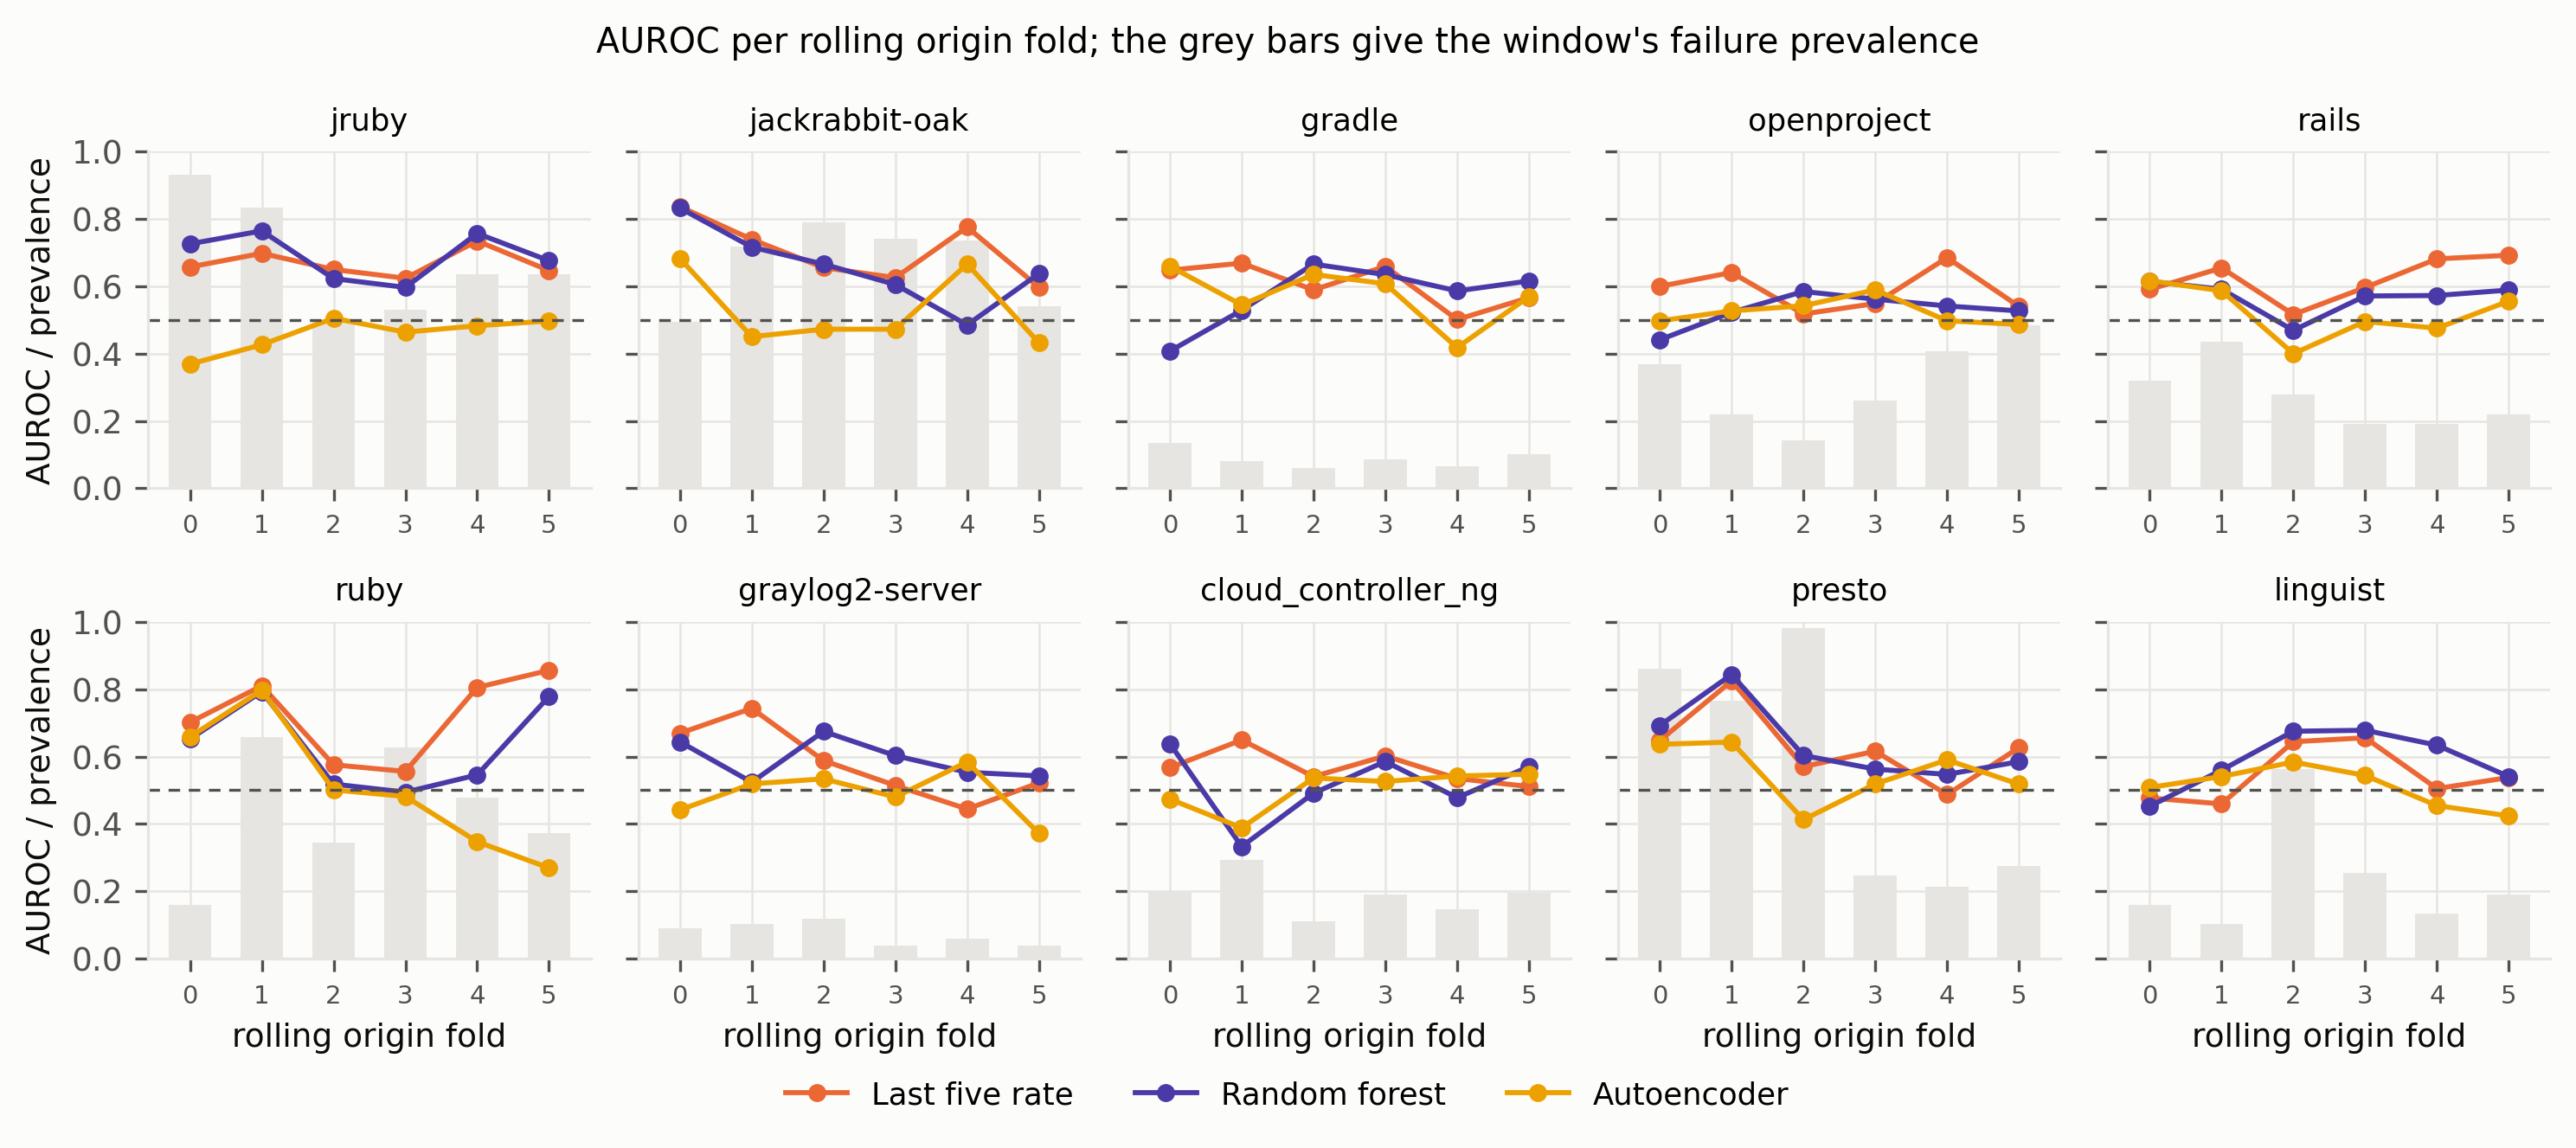
\includegraphics[width=0.78\linewidth]{fig_fold_trajectories.png}
  \caption{AUROC per rolling origin fold for LAST5, the random forest and the autoencoder, one panel per primary project; the grey bars give the failure prevalence of each test window.}
  \label{fig:folds}
\end{figure}

\paragraph{Autoencoder repair.} Table~\ref{tab:ae_repair} compares the legacy and repaired score. Under legacy weighting, one feature carries 13--72\% of reconstruction error (49\% mean); in seven projects it is constant among passing training builds. After repair, the largest feature share is 9--31\% (18\% mean). AUROC remains near chance (0.517 overall), indicating limited value in the repaired 44-feature novelty score. Isolation forest on history alone reaches 0.614.

\begin{table*}[htbp]
\centering
\footnotesize\setlength{\tabcolsep}{2.4pt}
\caption{Autoencoder Weighting Repair}
\label{tab:ae_repair}
\begin{tabular}{lrlrlrrr}
\toprule
Project & Zero var. & Legacy top feature & Share & Repaired top feature & Share & AUROC legacy & AUROC repaired \\
\midrule
jruby & 2 & gh\_tests\_deleted & 58\% & gh\_num\_commits\_on\_files\_touched & 9\% & 0.565 & 0.497 \\
jackrabbit-oak & 3 & gh\_description\_complexity & 44\% & gh\_tests\_added & 17\% & 0.515 & 0.432 \\
gradle & 0 & gh\_tests\_added & 13\% & gh\_test\_cases\_per\_kloc & 11\% & 0.561 & 0.569 \\
openproject & 2 & gh\_tests\_deleted & 62\% & gh\_team\_size & 14\% & 0.484 & 0.487 \\
rails & 2 & gh\_tests\_deleted & 50\% & git\_num\_all\_built\_commits & 16\% & 0.525 & 0.556 \\
ruby & 4 & gh\_description\_complexity & 49\% & gh\_files\_deleted & 17\% & 0.392 & 0.269 \\
graylog2-server & 2 & gh\_description\_complexity & 72\% & gh\_other\_files & 12\% & 0.184 & 0.372 \\
cloud\_controller\_ng & 2 & gh\_tests\_deleted & 53\% & gh\_sloc & 25\% & 0.563 & 0.548 \\
presto & 0 & gh\_team\_size & 31\% & gh\_team\_size & 31\% & 0.517 & 0.518 \\
linguist & 3 & hist\_n\_finished\_w10 & 62\% & gh\_files\_modified & 25\% & 0.498 & 0.424 \\
\bottomrule
\end{tabular}
\end{table*}



\paragraph{Answer.} Outcome history carries the signal; queue and duration telemetry, churn and repository attributes add nothing to it for any detector, and the repository attributes subtract from the supervised detectors by acting as time proxies. Prevalence moves by up to 0.77 between windows of the same project, learnt rankings invert when it does, and the rules are robust to it because they carry no learnt state.

\subsection{RQ4: What does the ranking quality buy at a matched operating point?}
\label{sec:results-rq4}

\begin{table*}[htbp]
\centering
\footnotesize\setlength{\tabcolsep}{3.5pt}
\caption{Threshold Operating Points}
\label{tab:operating}
\begin{tabular}{lrrrrrrrrr}
\toprule
 & \multicolumn{4}{c}{Native threshold} & \multicolumn{2}{c}{Matched budget (10\%)} & \multicolumn{3}{c}{Rolling threshold} \\
\cmidrule(lr){2-5} \cmidrule(lr){6-7} \cmidrule(lr){8-10}
Scorer & Alarm rate & Precision & Recall & Degenerate & Precision & Recall & Alarm rate & Precision & Recall \\
\midrule
Previous outcome & 0.350 & 0.472 & 0.467 & 0 & 0.506 & 0.171 &  & &  \\
Last five rate & 0.470 & 0.418 & 0.558 & 1 & 0.492 & 0.157 &  & &  \\
History LR & 0.396 & 0.446 & 0.501 & 1 & 0.504 & 0.171 &  & &  \\
Autoencoder & 0.211 & 0.371 & 0.230 & 0 & 0.392 & 0.119 & 0.144 & 0.384 & 0.165 \\
Isolation forest & 0.163 & 0.411 & 0.196 & 0 & 0.401 & 0.127 & 0.124 & 0.404 & 0.158 \\
PCA reconstruction & 0.128 & 0.363 & 0.131 & 0 & 0.371 & 0.105 & 0.108 & 0.352 & 0.113 \\
Random forest & 0.422 & 0.386 & 0.454 & 4 & 0.451 & 0.146 &  & &  \\
Gradient boosting & 0.441 & 0.381 & 0.474 & 2 & 0.428 & 0.135 &  & &  \\
\bottomrule
\end{tabular}
\end{table*}


\paragraph{Operating points.} Table~\ref{tab:operating} compares native and matched thresholds. Under native thresholds, supervised models flag 42--44\% of builds, unsupervised models 13--21\%, and rules 35--47\%; eight of 480 cells are degenerate. At the matched 10\% budget, precision is 0.49--0.51 for rules, 0.45 for random forest, 0.43 for gradient boosting, and 0.37--0.40 for unsupervised models, against prevalence 0.35. Rolling thresholds yield 11--14\% alarm rates for unsupervised models at similar precision.

\paragraph{Withhold scenario.} Tables~\ref{tab:cost_sweep} and \ref{tab:cost_project} show sensitivity to false-alarm cost and project-level outcomes. At two minutes, every scorer has positive median net savings of 2--5 compute minutes per build and eight of ten projects are positive. At a one-build false-alarm cost, median savings fall to 0.02 minutes for random forest, 0.3 for gradient boosting, and 0.9--1.2 for rules; only five or six projects remain positive. \proj{jruby/jruby} dominates savings because builds average 176 wall-clock minutes across nearly twenty jobs; \proj{rails/rails} and \proj{opf/openproject} also remain positive at one-build cost, while low-prevalence projects do not.

Compute-based savings can reward ranking expensive builds rather than predicting failures: unsupervised detectors have higher median savings at low false-alarm cost despite lower precision. At higher false-alarm costs, supervised detectors have the lowest median savings across scorers.

\begin{table}[htbp]
\centering
\scriptsize\setlength{\tabcolsep}{1.5pt}
\caption{Withhold Cost Sensitivity}
\label{tab:cost_sweep}
\begin{tabular}{lrrrrrrr}
\toprule
Scorer & 2 min & 5 min & 15 min & 30 min & 1 build & \shortstack{Positive\\at 2 min} & \shortstack{Positive\\at 1 build} \\
\midrule
Previous outcome & 3.25 & 3.17 & 2.93 & 2.57 & 1.20 & 8/10 & 6/10 \\
Last five rate & 3.25 & 3.18 & 2.93 & 2.44 & 0.96 & 8/10 & 5/10 \\
History LR & 3.09 & 3.02 & 2.79 & 2.34 & 0.86 & 8/10 & 6/10 \\
Autoencoder & 4.47 & 4.30 & 3.66 & 2.68 & 0.81 & 8/10 & 5/10 \\
Isolation forest & 4.92 & 4.81 & 4.47 & 3.56 & 1.12 & 8/10 & 6/10 \\
PCA reconstruction & 3.50 & 3.34 & 2.64 & 1.60 & 0.18 & 8/10 & 5/10 \\
Random forest & 1.82 & 1.74 & 1.47 & 1.06 & 0.02 & 8/10 & 5/10 \\
Gradient boosting & 2.07 & 1.97 & 1.65 & 1.17 & 0.33 & 8/10 & 5/10 \\
\bottomrule
\end{tabular}
\end{table}

\begin{table*}[htbp]
\centering
\footnotesize\setlength{\tabcolsep}{2.4pt}
\caption{Project Withhold Outcomes}
\label{tab:cost_project}
\begin{tabular}{lrrrrrrrrrrr}
\toprule
Project & Build & Prec. & \multicolumn{3}{c}{LAST5} & \multicolumn{3}{c}{RF} & \multicolumn{3}{c}{AE} \\
\cmidrule(lr){4-6} \cmidrule(lr){7-9} \cmidrule(lr){10-12}
 & (min) & LAST5 & Net 2 min & Net 1 build & Break even & Net 2 min & Net 1 build & Break even & Net 2 min & Net 1 build & Break even \\
\midrule
jruby & 176 & 0.85 & 1{,}067{,}647 & 1{,}055{,}877 & $>$9{,}999 & 1{,}010{,}820 & 997{,}126 & $>$9{,}999 & 1{,}303{,}699 & 1{,}281{,}832 & $>$9{,}999 \\
jackrabbit-oak & 40 & 0.82 & 12{,}248 & 10{,}151 & 87 & 2{,}472 & 832 & 51 & 19{,}228 & 16{,}236 & 43 \\
gradle & 17 & 0.19 & -358 & -3{,}042 & 0 & -490 & -3{,}350 & 0 & -456 & -3{,}306 & 0 \\
openproject & 122 & 0.45 & 81{,}798 & 67{,}933 & 578 & 69{,}514 & 52{,}365 & 379 & 67{,}322 & 50{,}563 & 417 \\
rails & 273 & 0.45 & 282{,}270 & 257{,}276 & 3{,}485 & 484{,}987 & 457{,}984 & 4{,}154 & 467{,}056 & 438{,}710 & 4{,}526 \\
ruby & 26 & 0.69 & 4{,}450 & 3{,}441 & 100 & 4{,}649 & 3{,}088 & 57 & 4{,}930 & 3{,}043 & 52 \\
graylog2-server & 18 & 0.16 & -215 & -2{,}200 & 0 & -295 & -2{,}327 & 0 & -261 & -2{,}440 & 0 \\
cloud\_controller\_ng & 96 & 0.31 & 7{,}321 & -373 & 53 & 9{,}789 & -1{,}952 & 59 & 8{,}772 & -2{,}995 & 42 \\
presto & 34 & 0.67 & 854 & -578 & 5 & 716 & -674 & 23 & 812 & -788 & 5 \\
linguist & 8 & 0.33 & 196 & -267 & 2 & 208 & -266 & 5 & 250 & -319 & 2 \\
\bottomrule
\end{tabular}
\end{table*}



\paragraph{Skip scenario.} Table~\ref{tab:skip} evaluates the intervention the build selection literature actually studies~\cite{jin2020, jin2022, abdalkareem2021skip}: the half of each test window with the lowest scores is skipped. A random ranking would skip half of the failures. The rules skip 40 to 41 percent of them while avoiding 37 percent of the window's compute; the random forest skips 43 percent of failures for 35 percent of compute, and the unsupervised detectors 46 to 49 percent for 32 to 33 percent, close to random. The median per project net saving is 22 to 23 compute minutes per build for the rules when a late observed failure costs 30 minutes and 14 to 15 when it costs 120 minutes, against 20 and 11 for the random forest. The ordering of scorers is the same as under every other view of the data, and the trade off is the one Jin and Servant describe: the compute saved is bought with failures observed late, and the ranking quality available here moves the exchange rate from one half to about two fifths.

\begin{table}[htbp]
\centering
\scriptsize\setlength{\tabcolsep}{2pt}
\caption{Build Skip Outcomes}
\label{tab:skip}
\begin{tabular}{lrrrrr}
\toprule
Scorer & Missed & Saved & Net: 30m & Net: 120m & Net: 1 build \\
\midrule
Previous outcome & 40.7\% & 37.2\% & 22.69 & 14.79 & 23.31 \\
Last five rate & 40.9\% & 37.0\% & 22.81 & 14.85 & 23.42 \\
History LR & 39.8\% & 37.1\% & 22.17 & 14.14 & 22.75 \\
Autoencoder & 48.6\% & 31.9\% & 14.17 & 8.70 & 14.65 \\
Isolation forest & 45.6\% & 33.0\% & 16.62 & 9.13 & 17.16 \\
PCA reconstruction & 47.4\% & 32.3\% & 15.32 & 8.56 & 15.79 \\
Random forest & 43.3\% & 34.8\% & 19.81 & 10.63 & 20.39 \\
Gradient boosting & 44.0\% & 34.4\% & 17.98 & 9.59 & 18.48 \\
\bottomrule
\end{tabular}
\end{table}



\paragraph{Answer.} At a matched alert budget the rules are the most precise scorers, at about half of flagged builds failing against a base rate of a third. Whether that buys anything depends on the intervention and the project, not on the detector. Withholding or deprioritising predicted failures pays only on projects with long, multi job builds and high prevalence, and only if a false alarm costs less than a project specific break even that is zero on the two low prevalence projects. Skipping the lower half of builds by predicted risk saves 37 percent of compute and observes 40 percent of failures late, against 50 percent for a random choice; the rules are again the best ranker for it.

\subsection{Robustness: the omitted projects, the single cut and the strict label}
\label{sec:results-robustness}

\begin{table}[htbp]
\centering
\scriptsize\setlength{\tabcolsep}{1.5pt}
\caption{Robustness Checks}
\label{tab:robustness}
\begin{tabular}{lrrrrr}
\toprule
Scorer & Primary 10 & Omitted 4 & All 14 & Single cut & Strict label \\
\multicolumn{6}{l}{\scriptsize Cells report AUROC / AUPRC lift.} \\
\midrule
Previous outcome & 0.627/1.46 & 0.688/2.02 & 0.644/1.62 & 0.624/1.34 & 0.628/1.47 \\
Last five rate & 0.623/1.41 & 0.677/1.87 & 0.638/1.54 & 0.622/1.32 & 0.625/1.42 \\
History LR & 0.630/1.48 & 0.694/2.06 & 0.648/1.65 & 0.633/1.37 & 0.632/1.49 \\
Autoencoder & 0.517/1.15 & 0.565/1.31 & 0.531/1.20 & 0.504/1.05 & 0.519/1.16 \\
Isolation forest & 0.548/1.25 & 0.618/1.50 & 0.568/1.32 & 0.552/1.21 & 0.547/1.25 \\
PCA reconstruction & 0.523/1.12 & 0.546/1.23 & 0.530/1.15 & 0.518/1.07 & 0.522/1.12 \\
Random forest & 0.598/1.37 & 0.676/1.94 & 0.621/1.53 & 0.571/1.33 & 0.593/1.39 \\
Gradient boosting & 0.577/1.31 & 0.657/1.65 & 0.600/1.41 & 0.570/1.25 & 0.577/1.33 \\
\bottomrule
\end{tabular}
\end{table}




Table~\ref{tab:robustness} reports results for the primary ten, omitted four, all fourteen, the single split, and strict labels. Rules score better on the omitted projects (PREV AUROC 0.688; lift 2.02) and retain their ordering over all fourteen. Under the single split, rules reach 0.62--0.63 AUROC and random forest 0.571. Strict relabeling changes each AUROC by at most 0.005. These checks do not change the main conclusions.

\section{Discussion}
\label{sec:discussion}

\subsection{What the signal is}
\label{sec:discussion-signal}

The results show moderate predictability on this TravisTorrent snapshot, driven mainly by recent outcomes. Failures cluster: after a red build, the next is more likely to be red; after a green build, more likely green. This pattern is consistent with prior build-selection and history-aware prediction work~\cite{jin2020, jin2022, nili2017, chen2020buildfast}. Under an enqueue-time boundary, completion-time lags, and forward evaluation, the 44-feature detectors add little to outcome history.

These findings are consistent with prior work reporting lower performance under temporal evaluation~\cite{chen2020buildfast, lyu2021splitting}. Here, mean AUROC is about 0.63 and mean lift about 1.4.

\subsection{Why the learned detectors do not add to the rule}
\label{sec:discussion-why}

Repository attributes act as temporal proxies; removing them improves supervised scores. Prevalence shifts by up to 0.77 within projects, disadvantaging fixed classifiers, while recent-outcome rules adapt at each build. Noisy environmental and cascading failures also limit pre-execution prediction~\cite{gallaba2018, ghaleb2021noise}. Unsupervised anomaly scores add little, even after correcting the autoencoder's variance weighting.

\subsection{Operational implications}
\label{sec:discussion-practice}

Teams should compare build-failure models with recent-outcome rules under rolling-origin evaluation. Queue reordering and early notification appear more practical here than withholding or skipping builds; those interventions depend on project costs and tolerance for failures observed late. Report precision at a stated alert budget with project-specific break-even costs.

\section{Threats to Validity}
\label{sec:threats}

\paragraph{Construct validity.} Travis status mixes defects, flaky tests, environmental failures, cascades, and cancellations~\cite{gallaba2018, ghaleb2021noise, lampel2021}. Strict-label sensitivity preserves the ordering, but the snapshot lacks allowed-failure flags. Lift is mean per-project AUPRC/prevalence; cost results depend on the assumed 15-minute information cost.

\paragraph{Internal validity.} Histories combine push and pull-request branches; branch-aware histories may change results. Pull-request descriptions can change after builds. Hyperparameters and rolling-threshold settings are fixed, not tuned, so stronger configurations may narrow model gaps.

\paragraph{External validity.} Data cover fourteen active Java and Ruby Travis CI projects from 2011--2015, not small repositories or mobile, embedded, and data-science projects. Modern CI platforms provide different telemetry and failure processes; current performance must be re-evaluated there~\cite{decan2022actions, sun2024ravenbuild}.

\paragraph{Conclusion validity.} The block bootstrap treats folds as independent despite shared training data. Ten projects limit power; non-rejection and ties do not establish equivalence.

\section{Reproducibility}
\label{sec:repro}

The package provides snapshot extraction, build-level data, feature pipeline, eight scorers, experiment runner, table and figure scripts, and unit tests. Tables and figures regenerate from stored results; a full run takes about 25 minutes on eight cores.

\section{Conclusion}
\label{sec:conclusion}

Across fourteen TravisTorrent projects, recent outcomes provide moderate ranking quality (mean AUROC 0.62--0.63; lift 1.41--1.48 on ten primary projects). No learned detector has a significant AUROC win over LAST5 after Holm correction; RF has one AUPRC win and one loss. History carries most signal, and repository attributes can reduce supervised performance under drift. At a matched alert budget, simple rules are most precise; withholding failures remains project- and cost-dependent.

The released package supports replication of this protocol and its baselines on newer CI platforms.

\begin{thebibliography}{99}

\bibitem{abdalkareem2021ml}
Rabe Abdalkareem, Suhaib Mujahid, and Emad Shihab. 2021.
A Machine Learning Approach to Improve the Detection of CI Skip Commits.
\textit{IEEE Transactions on Software Engineering} 47, 12 (2021). https://doi.org/10.1109/TSE.2019.2967380

\bibitem{abdalkareem2021skip}
Rabe Abdalkareem, Suhaib Mujahid, Emad Shihab, and Juergen Rilling. 2021.
Which Commits Can Be CI Skipped?
\textit{IEEE Transactions on Software Engineering} 47, 3 (2021). https://doi.org/10.1109/TSE.2019.2897300

\bibitem{aidasso2025slr}
Henri A\"{i}dasso, Mohammed Sayagh, and Francis Bordeleau. 2025.
Build Optimization: A Systematic Literature Review.
\textit{ACM Computing Surveys} 58, 1 (2025). https://doi.org/10.1145/3757912

\bibitem{beller2017oops}
Moritz Beller, Georgios Gousios, and Andy Zaidman. 2017.
Oops, My Tests Broke the Build: An Explorative Analysis of Travis CI with GitHub.
In \textit{Proceedings of the 14th International Conference on Mining Software Repositories (MSR 2017)}. IEEE. https://doi.org/10.1109/MSR.2017.62

\bibitem{beller2017travistorrent}
Moritz Beller, Georgios Gousios, and Andy Zaidman. 2017.
TravisTorrent: Synthesizing Travis CI and GitHub for Full Stack Research on Continuous Integration.
In \textit{Proceedings of the 14th International Conference on Mining Software Repositories (MSR 2017)}. IEEE. https://doi.org/10.1109/MSR.2017.24

\bibitem{chandola2009}
Varun Chandola, Arindam Banerjee, and Vipin Kumar. 2009.
Anomaly Detection: A Survey.
\textit{ACM Computing Surveys} 41, 3 (2009), Article 15. https://doi.org/10.1145/1541880.1541882

\bibitem{chen2020buildfast}
Bihuan Chen, Linlin Chen, Chen Zhang, and Xin Peng. 2020.
BuildFast: History Aware Build Outcome Prediction for Fast Feedback and Reduced Cost in Continuous Integration.
In \textit{Proceedings of the 35th IEEE/ACM International Conference on Automated Software Engineering (ASE 2020)}. ACM. https://doi.org/10.1145/3324884.3416616

\bibitem{davis2006}
Jesse Davis and Mark Goadrich. 2006.
The Relationship Between Precision Recall and ROC Curves.
In \textit{Proceedings of the 23rd International Conference on Machine Learning (ICML 2006)}. ACM. https://doi.org/10.1145/1143844.1143874

\bibitem{decan2022actions}
Alexandre Decan, Tom Mens, Pooya Rostami Mazrae, and Mehdi Golzadeh. 2022.
On the Use of GitHub Actions in Software Development Repositories.
In \textit{Proceedings of the IEEE International Conference on Software Maintenance and Evolution (ICSME 2022)}. IEEE.

\bibitem{durieux2019}
Thomas Durieux, Rui Abreu, Martin Monperrus, Tegawend\'{e} F. Bissyand\'{e}, and Lu\'{i}s Cruz. 2019.
An Analysis of 35+ Million Jobs of Travis CI.
In \textit{Proceedings of the IEEE International Conference on Software Maintenance and Evolution (ICSME 2019)}. IEEE. https://doi.org/10.1109/ICSME.2019.00044

\bibitem{elbaum2014}
Sebastian Elbaum, Gregg Rothermel, and John Penix. 2014.
Techniques for Improving Regression Testing in Continuous Integration Development Environments.
In \textit{Proceedings of the 22nd ACM SIGSOFT International Symposium on Foundations of Software Engineering (FSE 2014)}. ACM. https://doi.org/10.1145/2635868.2635910

\bibitem{falessi2020}
Davide Falessi, Jacky Huang, Likhita Narayana, Jennifer Fong Thai, and Burak Turhan. 2020.
On the Need of Preserving Order of Data When Validating Within Project Defect Classifiers.
\textit{Empirical Software Engineering} 25 (2020). https://doi.org/10.1007/s10664-020-09868-x

\bibitem{gallaba2018}
Keheliya Gallaba, Christian Macho, Martin Pinzger, and Shane McIntosh. 2018.
Noise and Heterogeneity in Historical Build Data: An Empirical Study of Travis CI.
In \textit{Proceedings of the 33rd ACM/IEEE International Conference on Automated Software Engineering (ASE 2018)}. ACM. https://doi.org/10.1145/3238147.3238171

\bibitem{gama2014}
Jo\~{a}o Gama, Indr\.{e} \v{Z}liobait\.{e}, Albert Bifet, Mykola Pechenizkiy, and Abdelhamid Bouchachia. 2014.
A Survey on Concept Drift Adaptation.
\textit{ACM Computing Surveys} 46, 4 (2014), Article 44. https://doi.org/10.1145/2523813

\bibitem{ghaleb2021noise}
Taher Ahmed Ghaleb, Daniel Alencar da Costa, Ying Zou, and Ahmed E. Hassan. 2021.
Studying the Impact of Noises in Build Breakage Data.
\textit{IEEE Transactions on Software Engineering} 47, 9 (2021). https://doi.org/10.1109/TSE.2019.2941880

\bibitem{hassan2006}
Ahmed E. Hassan and Ken Zhang. 2006.
Using Decision Trees to Predict the Certification Result of a Build.
In \textit{Proceedings of the 21st IEEE/ACM International Conference on Automated Software Engineering (ASE 2006)}. IEEE. https://doi.org/10.1109/ASE.2006.65

\bibitem{hassanwang2017}
Foyzul Hassan and Xiaoyin Wang. 2017.
Change Aware Build Prediction Model for Stall Avoidance in Continuous Integration.
In \textit{Proceedings of the ACM/IEEE International Symposium on Empirical Software Engineering and Measurement (ESEM 2017)}. IEEE. https://doi.org/10.1109/ESEM.2017.23

\bibitem{hilton2016}
Michael Hilton, Timothy Tunnell, Kai Huang, Darko Marinov, and Danny Dig. 2016.
Usage, Costs, and Benefits of Continuous Integration in Open Source Projects.
In \textit{Proceedings of the 31st IEEE/ACM International Conference on Automated Software Engineering (ASE 2016)}. ACM. https://doi.org/10.1145/2970276.2970358

\bibitem{holm1979}
Sture Holm. 1979.
A Simple Sequentially Rejective Multiple Test Procedure.
\textit{Scandinavian Journal of Statistics} 6, 2 (1979).

\bibitem{hong2024atlassian}
Yang Hong, Chakkrit Tantithamthavorn, Jirat Pasuksmit, Patanamon Thongtanunam, Arik Friedman, Xing Zhao, and Anton Krasikov. 2024.
Practitioners' Challenges and Perceptions of CI Build Failure Predictions at Atlassian.
In \textit{Companion Proceedings of the 32nd ACM International Conference on the Foundations of Software Engineering (FSE Companion 2024)}. ACM. https://doi.org/10.1145/3663529.3663856

\bibitem{jimenez2019}
Matthieu Jimenez, Renaud Rwemalika, Mike Papadakis, Federica Sarro, Yves Le Traon, and Mark Harman. 2019.
The Importance of Accounting for Real World Labelling When Predicting Software Vulnerabilities.
In \textit{Proceedings of the 27th ACM Joint Meeting on European Software Engineering Conference and Symposium on the Foundations of Software Engineering (ESEC/FSE 2019)}. ACM. https://doi.org/10.1145/3338906.3338941

\bibitem{jin2020}
Xianhao Jin and Francisco Servant. 2020.
A Cost Efficient Approach to Building in Continuous Integration.
In \textit{Proceedings of the ACM/IEEE 42nd International Conference on Software Engineering (ICSE 2020)}. ACM. https://doi.org/10.1145/3377811.3380437

\bibitem{jin2022}
Xianhao Jin and Francisco Servant. 2022.
Which Builds Are Really Safe to Skip? Maximizing Failure Observation for Build Selection in Continuous Integration.
\textit{Journal of Systems and Software} 188 (2022), 111292. https://doi.org/10.1016/j.jss.2022.111292

\bibitem{kapoor2023}
Sayash Kapoor and Arvind Narayanan. 2023.
Leakage and the Reproducibility Crisis in Machine Learning Based Science.
\textit{Patterns} 4, 9 (2023), 100804. https://doi.org/10.1016/j.patter.2023.100804

\bibitem{kerzazi2014}
Noureddine Kerzazi, Foutse Khomh, and Bram Adams. 2014.
Why Do Automated Builds Break? An Empirical Study.
In \textit{Proceedings of the IEEE International Conference on Software Maintenance and Evolution (ICSME 2014)}. IEEE. https://doi.org/10.1109/ICSME.2014.26

\bibitem{kunsch1989}
Hans R. K\"{u}nsch. 1989.
The Jackknife and the Bootstrap for General Stationary Observations.
\textit{The Annals of Statistics} 17, 3 (1989). https://doi.org/10.1214/aos/1176347265

\bibitem{lampel2021}
Johannes Lampel, Sascha Just, Sven Apel, and Andreas Zeller. 2021.
When Life Gives You Oranges: Detecting and Diagnosing Intermittent Job Failures at Mozilla.
In \textit{Proceedings of the 29th ACM Joint Meeting on European Software Engineering Conference and Symposium on the Foundations of Software Engineering (ESEC/FSE 2021)}. ACM. https://doi.org/10.1145/3468264.3473931

\bibitem{liu2008}
Fei Tony Liu, Kai Ming Ting, and Zhi-Hua Zhou. 2008.
Isolation Forest.
In \textit{Proceedings of the Eighth IEEE International Conference on Data Mining (ICDM 2008)}. IEEE. https://doi.org/10.1109/ICDM.2008.17

\bibitem{luo2014}
Qingzhou Luo, Farah Hariri, Lamyaa Eloussi, and Darko Marinov. 2014.
An Empirical Analysis of Flaky Tests.
In \textit{Proceedings of the 22nd ACM SIGSOFT International Symposium on Foundations of Software Engineering (FSE 2014)}. ACM. https://doi.org/10.1145/2635868.2635920

\bibitem{lyu2022interpretation}
Yingzhe Lyu, Gopi Krishnan Rajbahadur, Dayi Lin, Boyuan Chen, and Zhen Ming (Jack) Jiang. 2022.
Towards a Consistent Interpretation of AIOps Models.
\textit{ACM Transactions on Software Engineering and Methodology} 31, 1 (2022), Article 16. https://doi.org/10.1145/3488269

\bibitem{lyu2021splitting}
Yingzhe Lyu, Heng Li, Mohammed Sayagh, Zhen Ming (Jack) Jiang, and Ahmed E. Hassan. 2021.
An Empirical Study of the Impact of Data Splitting Decisions on the Performance of AIOps Solutions.
\textit{ACM Transactions on Software Engineering and Methodology} 30, 4 (2021), Article 54. https://doi.org/10.1145/3447876

\bibitem{mcintosh2018}
Shane McIntosh and Yasutaka Kamei. 2018.
Are Fix Inducing Changes a Moving Target? A Longitudinal Case Study of Just in Time Defect Prediction.
\textit{IEEE Transactions on Software Engineering} 44, 5 (2018). https://doi.org/10.1109/TSE.2017.2693980

\bibitem{nili2017}
Ansong Ni and Ming Li. 2017.
Cost Effective Build Outcome Prediction Using Cascaded Classifiers.
In \textit{Proceedings of the 14th International Conference on Mining Software Repositories (MSR 2017)}. IEEE. https://doi.org/10.1109/MSR.2017.26

\bibitem{olewicki2022}
Doriane Olewicki, Mathieu Nayrolles, and Bram Adams. 2022.
Towards Language Independent Brown Build Detection.
In \textit{Proceedings of the 44th International Conference on Software Engineering (ICSE 2022)}. ACM. https://doi.org/10.1145/3510003.3510122

\bibitem{politis1994}
Dimitris N. Politis and Joseph P. Romano. 1994.
The Stationary Bootstrap.
\textit{Journal of the American Statistical Association} 89, 428 (1994). https://doi.org/10.1080/01621459.1994.10476870

\bibitem{rausch2017}
Thomas Rausch, Waldemar Hummer, Philipp Leitner, and Stefan Schulte. 2017.
An Empirical Analysis of Build Failures in the Continuous Integration Workflows of Java Based Open Source Software.
In \textit{Proceedings of the 14th International Conference on Mining Software Repositories (MSR 2017)}. IEEE. https://doi.org/10.1109/MSR.2017.54

\bibitem{ruff2021}
Lukas Ruff, Jacob R. Kauffmann, Robert A. Vandermeulen, Gr\'{e}goire Montavon, Wojciech Samek, Marius Kloft, Thomas G. Dietterich, and Klaus-Robert M\"{u}ller. 2021.
A Unifying Review of Deep and Shallow Anomaly Detection.
\textit{Proceedings of the IEEE} 109, 5 (2021). https://doi.org/10.1109/JPROC.2021.3052449

\bibitem{saidani2020}
Islem Saidani, Ali Ouni, Moataz Chouchen, and Mohamed Wiem Mkaouer. 2020.
Predicting Continuous Integration Build Failures Using Evolutionary Search.
\textit{Information and Software Technology} 128 (2020), 106392. https://doi.org/10.1016/j.infsof.2020.106392

\bibitem{saidani2022}
Islem Saidani, Ali Ouni, and Mohamed Wiem Mkaouer. 2022.
Improving the Prediction of Continuous Integration Build Failures Using Deep Learning.
\textit{Automated Software Engineering} 29, 1 (2022), Article 21. https://doi.org/10.1007/s10515-021-00319-5

\bibitem{saito2015}
Takaya Saito and Marc Rehmsmeier. 2015.
The Precision Recall Plot Is More Informative than the ROC Plot When Evaluating Binary Classifiers on Imbalanced Datasets.
\textit{PLoS ONE} 10, 3 (2015), e0118432. https://doi.org/10.1371/journal.pone.0118432

\bibitem{sun2024ravenbuild}
Gengyi Sun, Sarra Habchi, and Shane McIntosh. 2024.
RavenBuild: Context, Relevance, and Dependency Aware Build Outcome Prediction.
\textit{Proceedings of the ACM on Software Engineering} 1, FSE (2024), Article 45. https://doi.org/10.1145/3643771

\bibitem{tantithamthavorn2017}
Chakkrit Tantithamthavorn, Shane McIntosh, Ahmed E. Hassan, and Kenichi Matsumoto. 2017.
An Empirical Comparison of Model Validation Techniques for Defect Prediction Models.
\textit{IEEE Transactions on Software Engineering} 43, 1 (2017). https://doi.org/10.1109/TSE.2016.2584050

\bibitem{vassallo2017}
Carmine Vassallo, Gerald Schermann, Fiorella Zampetti, Daniele Romano, Philipp Leitner, Andy Zaidman, Massimiliano Di Penta, and Sebastiano Panichella. 2017.
A Tale of CI Build Failures: An Open Source and a Financial Organization Perspective.
In \textit{Proceedings of the IEEE International Conference on Software Maintenance and Evolution (ICSME 2017)}. IEEE. https://doi.org/10.1109/ICSME.2017.67

\bibitem{xiali2017}
Jing Xia and Yanhui Li. 2017.
Could We Predict the Result of a Continuous Integration Build? An Empirical Study.
In \textit{Proceedings of the IEEE International Conference on Software Quality, Reliability and Security Companion (QRS-C 2017)}. IEEE. https://doi.org/10.1109/QRS-C.2017.59

\end{thebibliography}

\end{document}
